\documentclass[11pt,a4paper,oneside]{article}
\renewcommand{\baselinestretch}{1.2}
\usepackage{sectsty,setspace,natbib,wasysym} 
\usepackage[top=1.00in, bottom=1.0in, left=1in, right=1.25in]{geometry} 
\usepackage{graphicx}
\usepackage{latexsym,amssymb,epsf} 
\usepackage{epstopdf}
\usepackage{amsmath}

\newenvironment{smitemize}{
\begin{itemize}
  \setlength{\itemsep}{1pt}
  \setlength{\parskip}{0pt}
  \setlength{\parsep}{0pt}}
{\end{itemize}
}

\usepackage{fancyhdr}
\pagestyle{fancy}
\fancyhead[LO]{December 2013}
\fancyhead[RO]{Variable environments \& climate change}

\begin{document}
\renewcommand{\labelitemi}{$-$}
\title{Culled from: \\Coexistence and climate change: \\The role of
    temporal-variability in structuring future communities}
    \author{Wolkovich \& Donahue}
\date{Last updated: 13 December 2013}
\maketitle

\tableofcontents

\newpage
\section{Old ideas}

\subsection{Mortality \& phenology}

\noindent We also discussed mucking with \(m_{i}\) (the partial
mortality of species) to play around with
shifts in extreme events such as more frost dates following spring
warmth. But the above is more well-demonstrated or expected as
climate-related issues so we're not going there. (Note from Lizzie in
July 2011: I think this topic will be cool someday as it might be a
real issue in subalpine communities, but for now it's not for
sure. And given the equations we're using, it's not as crisp as the
above to get from \(environment\rightarrow m_{i}\). Note from Lizzie in October 2013: there is more on this now and it's been demonstrated for multiple communities. I have a literature review of this in the Appendix to my \emph{New Phytologist} Tansley paper if we ever want to look at this. But I continue to think it is still a touch ahead of its time (which, really, just means that everyone is already excited about it and thus working on it without good data, so once I go running after truly just hot topics, this would be the one to do! But, luckily, I am not there yet).)\\ 

\subsection{Correlated climate change variables}
\noindent \emph{From an old version of the abstract:} Specifically we examine how
synergistic effects of climate on multiple abiotic variables---for
example, earlier precipitation pulses and higher evapotranspiration
associated with earlier snowpack melting in the Sierras---alter
coexistence compared to single, unlinked variables ... We
  (might) find out that synergistic effects of multiple shifting
  abiotic variables reduce coexistence greater than single
  variables. \\

This was our big plan in July 2011, notes include:\\
\begin{itemize}
\item We compare the compounding effect of climate change: examining
  how shifts in single versus multiple environmental variables affect
  coexistence.
\item As of July 2011 I would say that the greatest interest in setting up
the paper lied in focusing on single vs. multiple variables, then
putting in tracking as subordinate. 
\end{itemize}

\noindent Old list of tasks on this I should make sure are thought through:
\begin{itemize}
\item Get on top of climate change lit: which variables will shift?
  Which ones are coupled and how will their coupling shift with
  climate change (go from uncoupled to coupled, or vice-versa, or just
  the coupling itself changes)?
\item Does evaporative stress increase with climate change (absolute,
  versus relative, oceans burn off while temperatures increase etc.)?
\item When seasons start earlier does evaporative stress increase (I
  suspect so, but need to pull together refs)?
\item Does lower snowpack mean earlier seasons?
\end{itemize}

\subsection{The endless debate about calculating drivers of coexistence, or not}
\emph{Do drivers of coexistence change with climate change? Schwing!}
\noindent We decided not to work on this (for now) as of October 2013 meeting. But then we did an about face and were all over it by the December 2013 meeting!\\

\noindent  {\bf Note:} Before our topic of interest was pretty damn significant: Do drivers of coexistence change with climate change (\emph{schwing! Sexy!})? So we should work this up, if not right away then soon after!\\

We decided on \emph{no analytical solutions} to storage effect versus relative nonlinearity (which are the main coexistence mechanisms), but we could do some of this conceptually post-simulations. We noted in October 2013 that even if we come up with these analytical solutions we'll still need an example, that is we would have to start with a community of \(n\) species that coexists via \(z\%\) relative non-linearity, \(x\%\) storage effect etc. and then we would impose climate change and see how \(z\%\) etc. change.\\

Again in October 2013: We again discussed the urge to partition out relative non-linearity and storage effect and how they will shift with climate change (fluctuation independent mechanisms seem less important here) but again we felt this was tricky and still depends on the simulations we run so we focused on how we will alter the equations to focus on shifts in the storage effect with climate change.

\subsection{Old equation for phenological tracking}
\noindent Old (pre 2012) vesion of adding phenological tracking to the model:
\begin{align*}
\hat{\tau_{i}} & = \tau_{p}-(\tau_{p}-\tau_{i})e^{-\alpha}
\end{align*}
\noindent thus, when:
\begin{align*}
& \alpha=0, \hat{\tau_{i}}=\tau_{i}
\\
& \alpha=\infty, \hat{\tau_{i}}=\tau_{p}
\end{align*}

\subsection{Old notes about trade-offs}
From October 2013:
\begin{itemize}
\item We have to create some species differences for the storage effect to `ameliorate' (EMW phrasing here, probably not ideal), so how do we want to do that?
\begin{itemize}
\item mean species differences in \(c_{i}\) and storage effect through \(g_{i}\) 
\item mean species differences in \(g_{max,i}\) and make them totally equivalent within season and temporal storage effect through \(\tau_{p}-\tau_{i}\) 
\end{itemize}

\noindent {\bf Stuff:} We will build in trade-offs (versus running a bunch of random parameter space models where---in order to get stability---we end up with related trade-offs) such that we're effectively saying `the world works this way now, we add climate change and see what happens. . . .' We think these trade-offs should be:
\begin{itemize}
\item decrease \(\phi_{i}\) correlated with  \(\tau_{i}\) close to  \(\tau_{p}\)
\item (for phenological tracking questions) decrease \(\phi_{i}\) correlated with higher tracking\footnote{though we could also alter \(c_{i}\) or \(u_{i}\), or might work better to adjust \(a_{i}\) so you can make earlier faster growers (or adjust \(a_{i}/u_{i}\) so when you're faster you're a higher R*), but we need to check through all this thinking more.}
\end{itemize}
Update as of 13 December 2013: We're off this idea because we are more interested in shifting variables related to R* if we are adding trade-offs in.\\

\noindent {\bf Question:} Should we add asymmetry in \(g_{i}\) such that \(\tau_{i}\) earlier than \(\tau_{p}\) is worse than \(\tau_{i}\) later than \(\tau_{p}\)? {\bf Answer: No!}

\subsection{How the growing season ends}
Worries over growing season continue (from August 2012 notes)! Worries over very short growing seasons (agree to stay with what we have for now, but keep in mind this possible issue and idea of continuous $R$ dripping in (or cyclically) for `growing season').\\

\noindent The intra-annual model does not have a useful closed solution (I
  have some Maxima code that shows only the trivial solution gives an
  equilibrium). This actually makes sense since the model is not a
  chemostat (a la Tilman \(R^{*}\)), we have a pulse that drains out
  and is not balanced by inputs.\\


\section{Notes from meeting with various people}

\subsection{Meeting with Jenn Williams}

\noindent 15 October 2013\\

\noindent  There are two big areas in modeling flowering reproduction stuff in plants:
\begin{enumerate}
\item When (which year) to reproduce
\item Bet-hedging across years (how much to reproduce)
\end{enumerate}

\noindent There is not much (anything of which she is aware) of when within a year to reproduce. She pointed out that this is probably because it's easy to measure how fitness varies year to year but there not very good estimates of how fitness varies with weather a species' phenology is early or late.\\

\noindent Once she said this I though 'right!' and this jives with my reading of the literature (especially late 1970s and early 1980s, culminating a little with Ollerton \& Lack's TREE paper). But, interestingly, climate change seems to be making this issue of how fitness correlates with phenology a critical topic (and something I realized I sort of work on, ugh). Also, Jeff Diez (new prof at Riverside) is doing some of this with a snowpack study he has started in the Alps (Levine lab).\\

++\\

\noindent Most of the models include multiple decisions. And almost models to date work on death as the cost of reproduction (her and Tom Miller are actually pioneering how to model non-lethal costs such as `if I reproduce I grow less').\\

\noindent How do models handle competition? They generally include density dependence in the seedling stage. Some sort of DD is necessary for any of the ESS (evolutionary stable strategy) models and everyone just tosses it in at the seedling stage.\\

\noindent Costs vs. trade-offs: costs manifest as trade-offs in many models. She thinks we should totally just toss in a trade-off and go for it. She does this a lot, she is just sure to apply the cost at several different doses (levels) although sometimes she only presents one level.\\

++\\

\noindent She doesn't know the plasticity literature, Pigliucci (looks like he's in UT-Knoxville, I think) does some very general theory and plasticity stuff. \\

\newpage
\subsection{Meeting with Sally Otto} 

\noindent 22 October 2013\\

\noindent Okay, so she didn't really answer my costs versus trade-offs question directly. She just dove in and suggested a new formulation with costs. She felt like a model that incurred mortality when germination occurred before the pulse would be better. You could then treat \(g_{i}\) possibly as a constant or such. I pointed out that \(g_{i}\) often creates \(covar(E,C)\) but I think her model may as well, but through the intra-annual part of the equation. I think there are probably other issues with her conceptualization as well (like how we would make tracking happen) but I haven't got there yet.\\

\noindent Let:
\begin{align*}
D & = \text{normal distribution representing time of germination of species }i\\
T & = \text{intra-annual time}
\end{align*}

\noindent Then, how about this (with a less funky equation for \(g_{i}\)):

\begin{align*}
N_{i}(t+1) & =
s_{i}(N_{i}(t)(1-g_{i})+N_{i}(t)g_{i}\phi_{i}\int_{D=\tau_{p}}^{\infty}norm(\mu_{p}, \sigma_{p})_{D} [\int_{T=D}^{t+\delta}B_{i}(T) \mathrm{d}T] \mathrm{d}D)
\end{align*}

\newpage
\section{Figure ideas from 2011}
\begin{figure}[h!]
\centering
\noindent 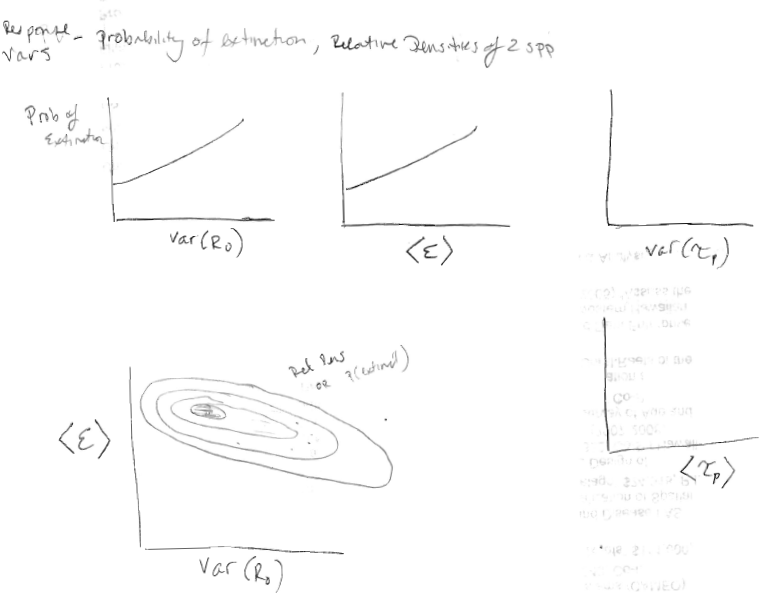
\includegraphics[width=1\textwidth]{/Users/Lizzie/Documents/git/temporalvar/figures/figurehopes_1.png}
\caption{{\bf Synergistic environmental effects (from 2011).}  Figure aspirations
  for part 1 of the paper, which covers how varying environmental
  variables (\(\tau_{p}\), \(R_{\theta}\), \(\epsilon\)) alone and in concert (as predicted by climate change)
  alters coexistence. Single variables will be simple graphs, while
  contour plots will come in for varying more than one variable
  together. (There is no phenological tracking by species in this
  section of the paper.) From July 2011 meeting.}
\end{figure}

\newpage
\begin{figure}[h!]
\centering
\noindent 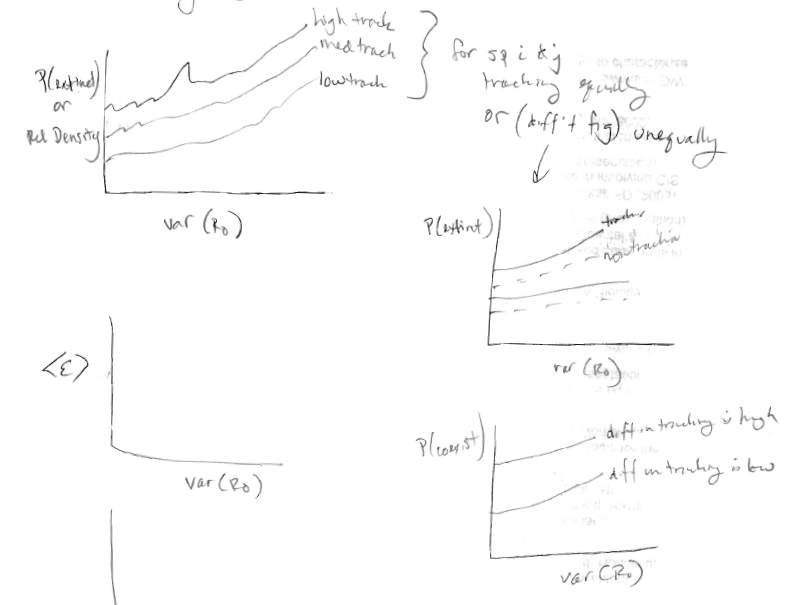
\includegraphics[width=1\textwidth]{/Users/Lizzie/Documents/git/temporalvar/figures/figurehopes_2.png}
\caption{{\bf Phenological tracking and coexistence under climate
    change (from 2011).}  We didn't quite nail these down: do we vary both species
so they both track or look at one tracking and one not tracking?
Hoping this will become clear as we get the model up and running. From July 2011 meeting.}
\end{figure}



\end{document}

